\clearpage
%%=========================================
\section{MCT Film Grown by MBE on  Substrate C}\label{sec:subCc}

A film of \acl{mct} was grown on substrate C by \ac{mbe}. 

\begin{figure}[htbp]
    \centering
    \mySubfigure{0.49\textwidth}{CMT801_om_bf_grid_14_10x.png}[fig:subCc_om_centre][angle=180]
    \hfill
    \mySubfigure{0.49\textwidth}{CMT801_om_bf_grid_21_10x.png}[fig:subCc_om_corner][angle=180]
    \caption[Bright field microscopy images of \ac{mct} film grown by \ac{mbe} on substrate AC]{Bright field microscopy images of \ac{mct} film grown by \ac{mbe} on (211)B-oriented substrate C: \subref{fig:subCc_om_centre} Near the centre; and \subref{fig:subCc_om_corner} near the lower left corner.}
    \label{fig:subCc_om}
\end{figure}

%%=========================================
\subsection{Particles}

\citet{selvig2007defects} describe the irregularly shaped defects with sizes extending from \SI{10}{\micro\metre} to a few hundred microns as high temperature voids and the ones with size less than \SI{10}{\micro\metre} as microvoids. These types of defects are typically formed during the growth of the material and the density is dependent on the deviation from ideal growth conditions. High temperature voids are formed at substrate temperatures higher than the \ce{Te}-phase limit, while microvoids are formed at low substrate temperature.

\todo{Sammenlign med telling av tellurium precipitates.}

\begin{figure}[htbp]
    \centering
    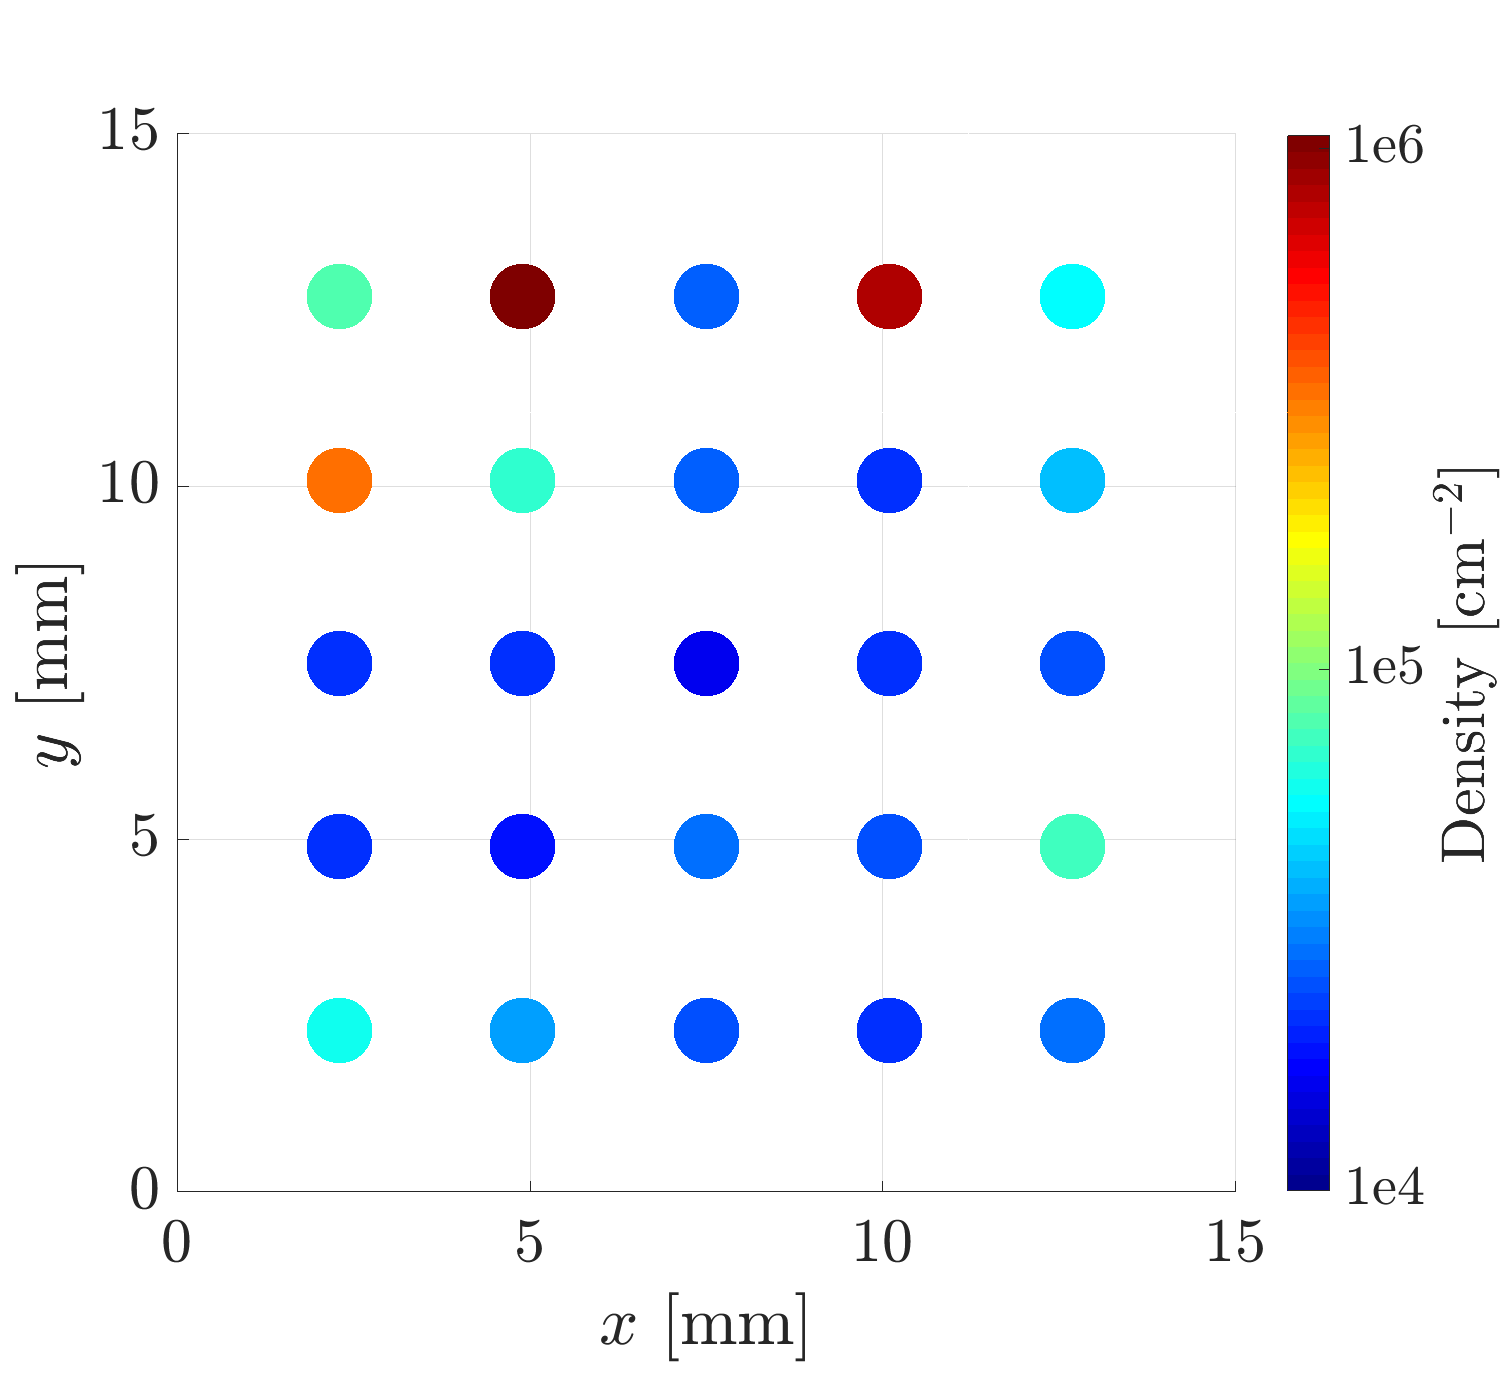
\includegraphics[width=0.5\linewidth]{CMT801_densityData.png}
    \caption[Map of the density of microvoids on the \ac{mct} film grown on substrate C.]{A map of the density of microvoids at 36 different locations on the $\SI{15}{\milli\metre}\times\SI{15}{\milli\metre}$ \ac{mct} film grown by \ac{mbe} on substrate C. The density measurements were obtained by counting the number of microvoids in bright field optical microscopy images covering $\SI{558}{\micro\metre}\times\SI{419}{\micro\metre}$ areas. In total, \SI{0.94}{\percent} of the substrate surface was measured. The density was observed to vary between \SIrange{4e+3}{6e+4}{\centi\metre^{-2}} with an average defect density of \SI{2e+04}{\centi\metre^{-2}}.}
    \label{fig:CMT801_densityData}
\end{figure}

The density of microvoids was found to be between \SIrange{2e+4}{1e+6}{\centi\metre^{-2}}. The average density was \SI{1e+05}{\centi\metre^{-2}} with a standard deviation of \SI{3e+05}{\centi\metre^{-2}}. A graphical representation of the density at different locations on the film can be seen in Fig.~\ref{fig:CMT801_densityData}. The sample Pearson correlation coefficient between the occurrence of polishing grit on the etched substrate C and the occurrence of microvoid defects on the film was determined to be \SI{0.33}{}, which was a weak positive correlation. The residue from the evaporation of a acetone droplet, which settled on the surface when removing the etched substrate from the \ac{sem} holder, was clearly visible in the layer as a formation of microvoids, as seen in Fig.~\ref{fig:subCc_microvoids_correlation}.

\begin{figure}[htbp]
    \centering
    \mySubfigure{0.49\linewidth}{subCb_om_df_n004_5x.png}[fig:subCb_om_df_n004_5x][angle=180]
    \hfill
    \mySubfigure{0.49\linewidth}{CMT801_om_bf_grid_04_10x-1.png}[fig:CMT801_om_bf_grid_04_10x-1][angle=180]
    \caption[Residue on etched substrate C visible as microvoids in the film.]{The residue from the evaporation of a acetone droplet on the etched substrate C was correlated with microvoids in the \ac{mct} film grown on substrate C: \subref{fig:subCb_om_df_n004_5x} Dark field microscopy image of etched substrate C; \subref{fig:CMT801_om_bf_grid_04_10x-1} bright field microscopy of \ac{mct} film.}\label{fig:subCc_microvoids_correlation}
\end{figure}


%%=========================================
\subsection{Composition and Thickness}

\Iac{ftir} transmission spectrum was recorded from one spot in the centre of the \ac{mct} film grown by \ac{mbe} on substrate C. The \ac{ir} transmittance was between \SI{50}{\percent} and \SI{63}{\percent} in the wavenumber range between \SIrange{400}{1400}{\centi\metre^{-1}}, see Fig.~\ref{fig:subCc_ftir}. The cut-on wavenumber was at \SI{1564.7}{\centi\metre^{-1}}, which corresponds to a wavelength of \SI{6.39}{\micro\metre}. Consequently, the $x$-value was \SI{0.224}{} according to the formula by \citet{bricexxxxtttt}. The thickness of the \ac{mct} film was calculated to be \SIrange{11.0}{11.6}{\micro\metre} by using Eq.~\ref{eq:ftir_thickness}.

\todo{FTIR: correlate with polishing grit or donut density.}

\begin{figure}[htbp]
    \centering
    \mySubfigure{0.60175438596\linewidth}{CMT801_ftir_spectra.png}[fig:subCc_ftir_spectra]
    \hfill
    \mySubfigure{0.37824561403\linewidth}{CMT801_ftir_transmission_at_k500cm-1.png}[fig:subCc_ftir_map_500cm-1]
    \caption[\Ac{ftir} measurement from one spot on the \ac{mct} film grown on substrate C.]{\Ac{ftir} measurements recorded from one spot on the $\SI{15}{\milli\metre}\times\SI{15}{\milli\metre}$ \ac{mct} film grown on substrate C: \subref{fig:subCc_ftir_spectra} Transmission spectrum; \subref{fig:subCc_ftir_map_500cm-1} transmission map at wavenumber $k=\SI{500}{\centi\metre^{-1}}$ showing the transmittance $T$ in percentage of incoming light at the point.}\label{fig:subCc_ftir}
\end{figure}

%%=========================================
\subsection{Impurity Analysis -- EDS}

\begin{comment}
\begin{table}[htbp]
    \centering
    \caption[\Ac{eds} impurity analysis of \ac{mct} film grown by \ac{mbe} on substrate C.]{Results of the \ac{eds} impurity analysis at three different locations on the $\SI{15}{\milli\metre}\times\SI{15}{\milli\metre}$  \ac{mct} film grown by \ac{mbe} on (211)B-oriented substrate C (atomic concentration \%). The X-ray signal is acquired from $\SI{1270}{\micro\metre}\times\SI{890}{\micro\metre}$ areas near the centre, upper edge, and upper left corner.}\label{tab:subBc_eds_analysis}
   \begin{tabu} to 1.0\textwidth { X[1.85, r] X[1.125,c] X[1.125,c] X[1.125,c] X[1.125,c] X[1.125,c] X[1.125,c] }
        \hline
            & \textbf{\ce{Te}} (at.\%) & \textbf{\ce{Hg}} (at.\%) & \textbf{\ce{Cd}} (at.\%) & \textbf{\ce{C} } (at.\%) & \textbf{\,\ce{O}\,} (at.\%) & \textbf{\ce{Al}} (at.\%) \\
        \hline
        Near centre & \SI{44,36}{} & \SI{31,14}{} & \SI{12,19}{} & \SI{11,30}{} & \SI{0,86}{} & \SI{0,16}{} \\
        Near edge & \SI{44,12}{} & \SI{32,26}{} & \SI{10,81}{} & \SI{11,49}{} & \SI{1,14}{} & \SI{0,18}{} \\
        Near corner & \SI{44,26}{} & \SI{32,58}{} & \SI{10,71}{} & \SI{11,23}{} & \SI{1,03}{} & \SI{0,19}{}  \\
        \hline
    \end{tabu}
\end{table}
\end{comment}

%%=========================================